\documentclass[a4paper]{article}
% Import some useful packages
\usepackage[margin=0.5in]{geometry} % narrow margins
\usepackage[utf8]{inputenc}
\usepackage[english]{babel}
\usepackage{hyperref}
\usepackage{bm}
\usepackage{listings}
\usepackage{amsmath,graphicx,varioref,verbatim,amsfonts,geometry,amssymb,dsfont,blindtext}
%\usepackage{minted}
\usepackage{amsmath}
\usepackage{xcolor}
\hypersetup{colorlinks=true}
\definecolor{LightGray}{gray}{0.95}
\definecolor{dkgreen}{rgb}{0,0.6,0}
\definecolor{gray}{rgb}{0.5,0.5,0.5}
\definecolor{mauve}{rgb}{0.58,0,0.82}
\definecolor{mygray}{rgb}{0.9,0.9,0.9}
\definecolor{LightGray}{gray}{0.95}
\lstset{frame=tb,
	language=Python,
	aboveskip=3mm,
	belowskip=3mm,
	showstringspaces=false,
	columns=flexible,
	basicstyle={\small\ttfamily},
	numbers=none,
	numberstyle=\tiny\color{gray},
	keywordstyle=\color{blue},
	commentstyle=\color{dkgreen},
	stringstyle=\color{mauve},
	backgroundcolor=\color{mygray}
	%breaklines=true,
	%breakatwhitespace=true,
	%tabsize=3
}
\title{Project 3 in FYS3150}
\author{Bendik Steinsvåg Dalen, Ulrik Seip}
%\renewcommand\thesection.\alph{section}
%\renewcommand\thesection{\Alph{section}}
\renewcommand\thesubsection{\thesection.\alph{subsection}}
\renewcommand\thesubsubsection{\thesubsection.\roman{subsubsection}}
\begin{document}
\maketitle

https://github.com/UlrikSeip/Projects/tree/master/prosjekt3

\section{ABSTRACT}
In this project we simulate the orbits of all the 8 planets in the solar system, and Pluto. Comparing the Forward Euler and the Velocity Verlet methods we find the Velocity Verlet method to be preferable due to its conservation of energy. We then test the Velocity Verlet method against the analytically derived escape velocity and perihelion of Mercury.

\section{INTRODUCTION}
Our solar system is littered with asteroids, planets and moons. This plethora objects floating around in space makes for a perfect exercise in solving multi body differential equations in 3 dimensions.

When simulating orbits for several celestial bodies with high accuracy, the computation can be expensive, and so it is paramount to strike a balance  between efficiency and accuracy. To explore this balance, we will run simulations using the Velocity-Verlet integration method, and comparing with the Forward-Euler method. Having found the optimal way to simulate the orbits, we move on to test the effect of the gravitational pull between planets, and complete a full model for all planets of the solar system, and Pluto. 

\section{METHOD}

\subsection{Newtons law of gravitation}
One of the most common representations of newtons law of gravitation on Earth is
\begin{align}
\boldsymbol{F}_{G} = \frac{M_{\text{Earth}}v^{2}}{r}\boldsymbol{\hat{r}} = \frac{GM_{\odot} M_{\text{Earth}}}{r^{2}}\boldsymbol{\hat{r}},
\end{align}
where $G=6.67\cdot10^-11\frac{m^3}{kgs^2}$ is the gravitational constant, $m_1$ and $m_2$ are the masses of the bodies exerting a force upon each other, $F_G$ is said force, and $r$ is the distance between the bodies. Using Keplers laws this can be further simplified to
\begin{align}
\boldsymbol{F}_G=\frac{{M_{\odot}M_\text{Earth}}4\pi^{2}}{r^{2}}\frac{\mathrm{AU}^{3}}{\mathrm{yr}^{2}}\boldsymbol{\hat{r}}.
\end{align}
We can then rewrite this for a point mass and acceleration as
\begin{align}
\boldsymbol{a}=\frac{{M_{\odot}}4\pi^{2}}{r^{2}}\frac{\mathrm{AU}^{3}}{\mathrm{yr}^{2}}\boldsymbol{\hat{r}}. \label{akselerasjon}
\end{align} 

\subsection{The Forward Euler method}
To use equation \ref{akselerasjon} for the Forward Euler method we need an expression for $\Delta \boldsymbol{v}$. We therefore introduce a time step $dt$. We also define $\boldsymbol{\hat{r}}=\cos(\theta)\boldsymbol{\hat{i}}+\sin(\theta)\boldsymbol{\hat{j}}+\cos(\phi)\boldsymbol{\hat{k}}$. This gives us
\begin{align*}
\frac{d\boldsymbol{v}}{dt}=\frac{v_{i+1}-v_i}{dt}=-4\pi^2\frac{M_{\odot}}{r^2}\boldsymbol{\hat{r}}
\end{align*}
\begin{align}
\boldsymbol{v}_{i+1}=-4\pi^2\frac{M_\odot}{r^2}dt\boldsymbol{\hat{r}} + \boldsymbol{v}_i 
= -\boldsymbol{a}_i dt  + \boldsymbol{v}_i.
\end{align}
We can do something similar to find $\Delta \boldsymbol{x}$:
\begin{align*}
\frac{d\boldsymbol{x}}{dt}=\frac{x_{i+1}-x_i}{dt} = v_{i+1}\boldsymbol{\hat{r}} = \boldsymbol{v}_{i+1}
\end{align*}
\begin{align}
\boldsymbol{x}_{i+1}= \boldsymbol{v}_{i+1}dt + \boldsymbol{x}_i 
= \boldsymbol{v}_{i+1} dt  + \boldsymbol{x}_i.
\end{align}



\subsection{The Velocity Verlet method}
From \cite{lecture notes} we know that the Verlet formula for a specific $x_i$ is
\begin{align}
x_{i+1} = 2x_i - x_{i-1} + h^2 x_i^{(2)} + O(h^4) \label{verlet},
\end{align}
where $h$ is the timestep, $x^{(2)}$ is function \ref{akselerasjon}, and $O$ is the truncation error. We also know that the velocity is
\begin{align}
x_i^{(1)} = \frac{x_{i+1} - x_{i-1}}{2h} + O(h^2). \label{vVerlet}
\end{align}
Unfortunaley function \ref{verlet} is a bit difficult to use as we only know the initial position, and thus can't find $x_1$ or $x_2$, and so forth. To help with this we can rewrite them into
\begin{align}
x_{i+1} = x_i + hx_i^{(1)} + \frac{h^2}{2}x_i^{(2)} \label{velVerlet}
\end{align}
and
\begin{align}
x_i^{(1)} = x_{i-1}^{(1)} + \frac{h}{2} \left( x_i^{(2)} + x_{x-i}^{(2)} \right) \label{VvelVerlet},
\end{align}
see section \ref{vVerlet_math} for more details.


\subsection{The code for the implementations}
Both the Velocity Verlet and the Forward Euler algorithms were implemented using a combination of python and Julia. Python happens to be a convenient language for making an object oriented implementation of a solar system simulation, while Julia is in most cases more than 10 times faster than Python, and even rivals c++, when it comes to computation speeds.


\subsection{Testing the algorithms}
To test our algorithm we can check if the escape velocity of our planets is correct. We find it analytically by using conservation of energy, and the fact that the kinetic energy, and the potential energy of our planets are defined with opposite signs. We therefore start with the equation:
\begin{align*}
E_k + E_p = \tfrac{1}{2}M_{E}v_{esc}^{2} - G\dfrac{M_{\odot}M_{E}}{r} = 0
\end{align*}
If we then isolate $v_{esc}$ on the left side of the equation, we end up with the following equation: 
\begin{align}
V_{esc} = \sqrt{\dfrac{2GM_{\odot}}{r}}
\end{align}
To test our implementation against the analytical solution we simply run a simulation for an imaginary planet with the initial analytical velocity, and see if it has returned after several thousand years. We can also try simulating with a slightly lower initial velocity, and se if the planet does indeed stay in orbit with anything less than the analytical initial velocity.

Furthermore the algorithms can be tested against each other for both accuracy and consistency.


\subsection{The three-body problem}
We now have a good basis to extend our algorithm to study the three-body problem, by adding Jupiter to the equation. The force between Earth and Jupiter is
\begin{align}
\boldsymbol{F}_{\text{Earth-Jupiter}} = \frac{G M_\text{Jupiter} M_{\text{Earth}}} {r_{\text{Earth-Jupiter}}^{2}} \boldsymbol{\hat{r}}.
\end{align}
For simplicity's sake we will keep the Sun fixed in the centre of mass, or origo, for now. For each timestep we then calculate the force on Earth and Jupiter from the Sun, and the the force between Earth and Jupiter, and add them up. We then get an position array for both Earth and Jupiter.

To test the stability of our Verlet solver we also studied what effect increasing the magnitude of Jupiter by 10 and 1000 would have on the system.


\subsection{Final model for all planets of the solar system}
We now almost have a working model of the solar system. Firstly we calculated the three-body problem of the Earth, Sun and Jupiter again, but now treating the Sun as an object, instead of fixing it in the centre of mass. We then get the path of the objects around the centre of mass. The initial values of the Sun was found by setting the posisiton in origo, and making sure the momentum of the Sun was the negative of the total momentum of the other planets. 

Finaly we simply added the remaining planets, and Pluto, to the calculation as extra bodies. The acceleration on each body was found as above, by calculating the force on each object from the other objects. 


\section{RESULTS}
\subsection{Testing the algorithms}
As can be seen in figure \ref{escape_vel} the planet did indeed escape with our analytical initial velocity, and figure \ref{nescape_vel} shows that a slight reduction to said initial velocity places the planet back in orbit.

When comparing the Velocity Verlet and Forward Euler algorithms we observe an increase in the orbits radius for both cases both in 2 and 3 dimensions. In figure \ref{fe2d}, \ref{vv2d}, \ref{fe3d}, \ref{vv3d} we observe a higher increase for the Forward Euler Method

\begin{figure}[h!]
	\centering 
	%Scale angir størrelsen på bildet. Bildefilen må ligge i %samme mappe som tex-filen. 
	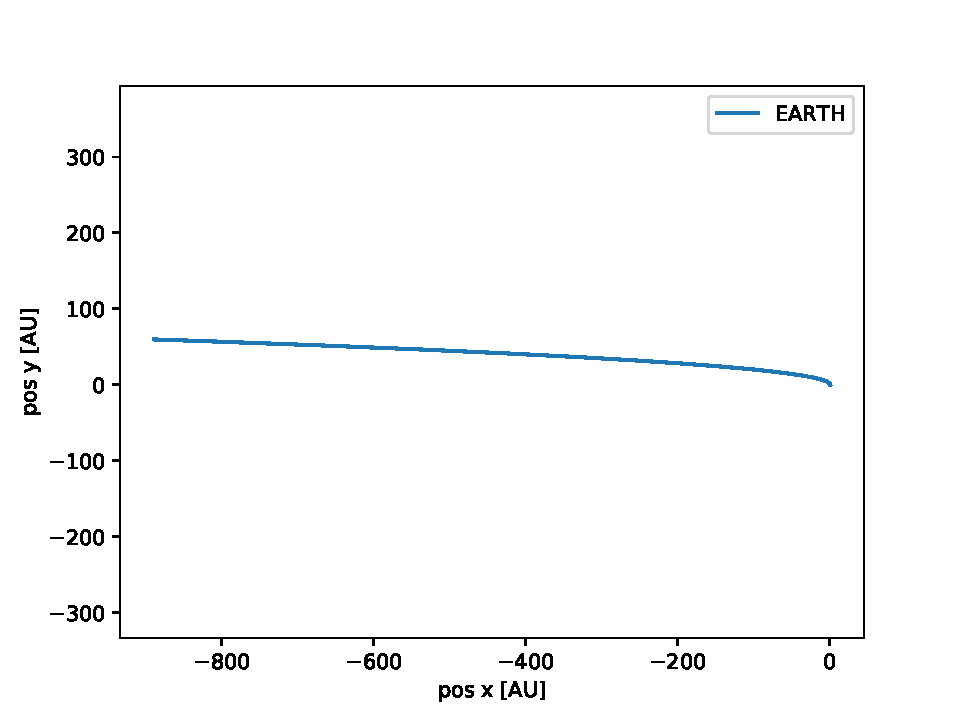
\includegraphics[scale=0.7]{escapeVelocity2000.pdf}
	\caption{A plot of the simulated minimal escape velocity over 2000 years}
	%Label gjør det enkelt å referere til ulike bilder.
	\label{escape_vel}
\end{figure}

\begin{figure}[h!]
	\centering 
	%Scale angir størrelsen på bildet. Bildefilen må ligge i %samme mappe som tex-filen. 
	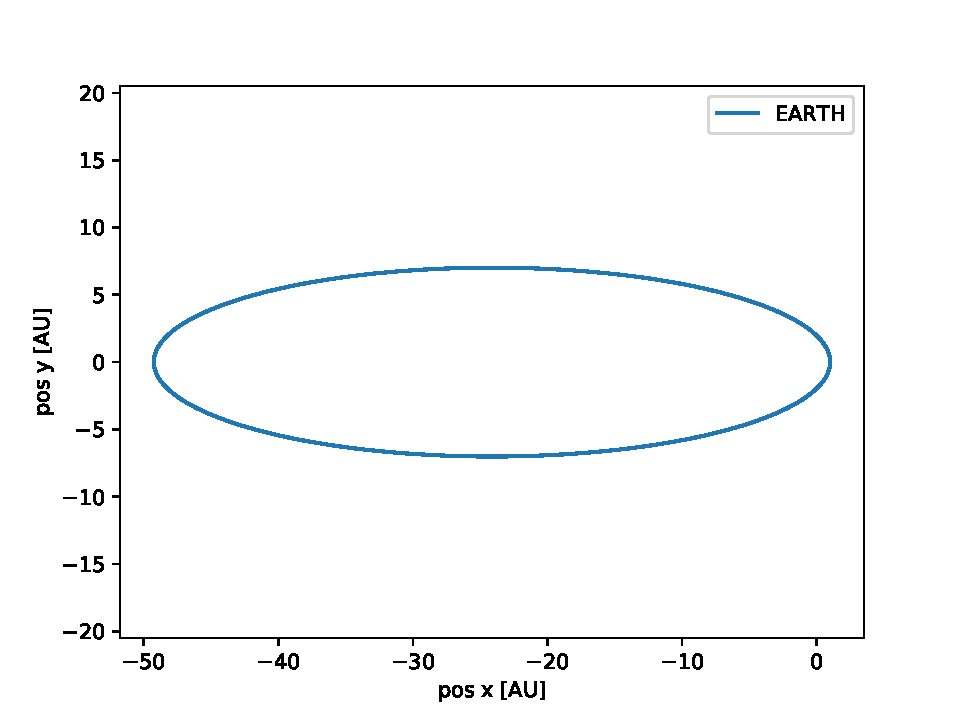
\includegraphics[scale=0.7]{allmostEscapeVelocity2000.pdf}
	\caption{Initial velocity at .99 if escape velocity over 2000 years}
	%Label gjør det enkelt å referere til ulike bilder.
	\label{nescape_vel}
\end{figure}

\begin{figure}[h!]
	\centering 
	%Scale angir størrelsen på bildet. Bildefilen må ligge i %samme mappe som tex-filen. 
	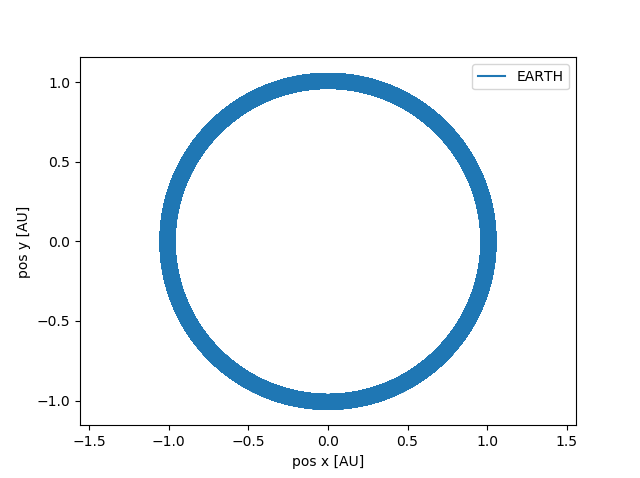
\includegraphics[scale=0.7]{fe1e4_2d.png}
	\caption{A 10000 year simulation with the forward euler method in 2d, $dt = \frac{1}{100}years$}
	%Label gjør det enkelt å referere til ulike bilder.
	\label{fe2d}
\end{figure}

\begin{figure}[h!]
	\centering 
	%Scale angir størrelsen på bildet. Bildefilen må ligge i %samme mappe som tex-filen. 
	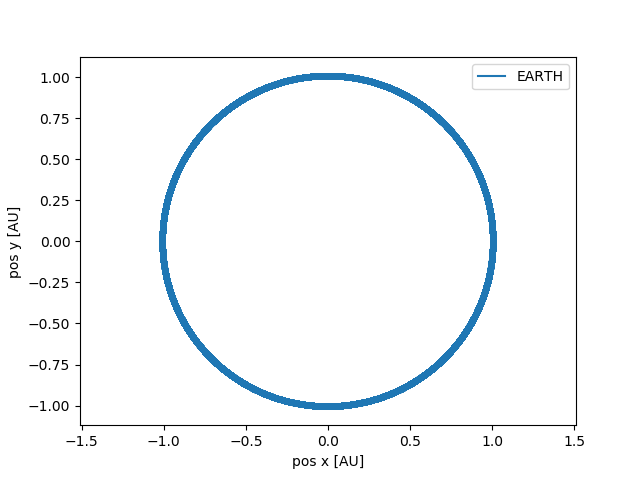
\includegraphics[scale=0.7]{vv1e4_2d.png}
	\caption{A 10000 year simulation with the velocity verlet method in 2d, $dt = \frac{1}{100}years$}
	%Label gjør det enkelt å referere til ulike bilder.
	\label{vv2d}
\end{figure}

\begin{figure}[h!]
	\centering 
	%Scale angir størrelsen på bildet. Bildefilen må ligge i %samme mappe som tex-filen. 
	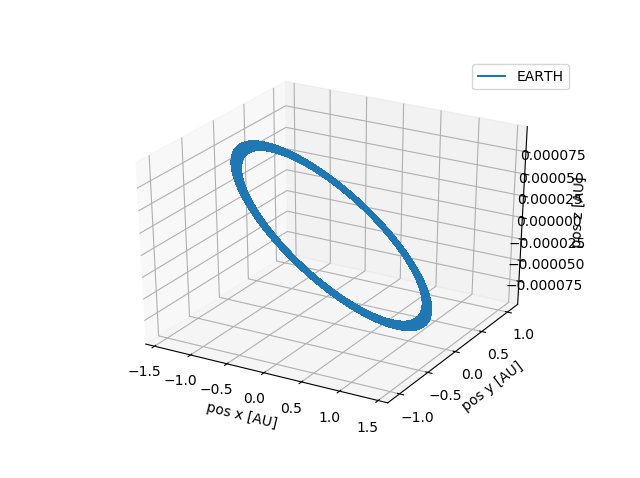
\includegraphics[scale=0.7]{fe1e4_3d.png}
	\caption{A 10000 year simulation with the forward euler method in 3d, $dt = \frac{1}{100}years$}
	%Label gjør det enkelt å referere til ulike bilder.
	\label{fe3d}
\end{figure}

\begin{figure}[h!]
	\centering 
	%Scale angir størrelsen på bildet. Bildefilen må ligge i %samme mappe som tex-filen. 
	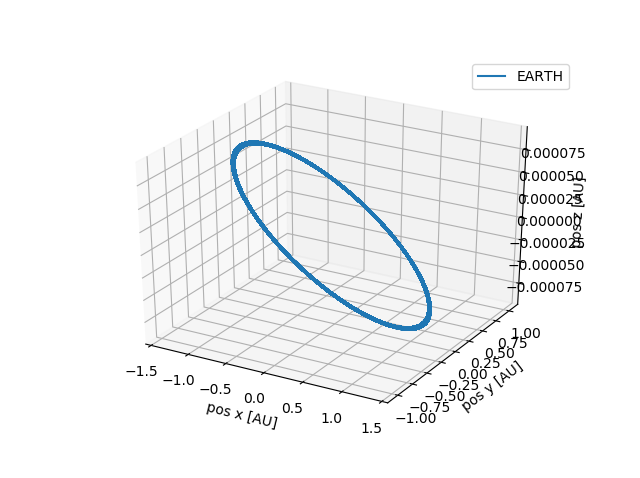
\includegraphics[scale=0.7]{vv1e4_3d.png}
	\caption{A 10000 year simulation with the velocity verlet method in 3d, $dt = \frac{1}{100}years$}
	%Label gjør det enkelt å referere til ulike bilder.
	\label{vv3d}
\end{figure}


\subsection{The three-body problem}
The plot of the path of Jupiter and Earth can be seen in figure \ref{e_1}, with an elapsed time of $t=30\text{yr}$ and a timestep of $10^{-5} \text{yr}$. The path when Jupiter has 10 and 1000 times more mass, with the same time interval, can be seen in figure \ref{e_10} and \ref{e_1000} respectively. 

\begin{figure}[h!]
		\centering 
		%Scale angir størrelsen på bildet. Bildefilen må ligge i samme mappe som tex-filen. 
		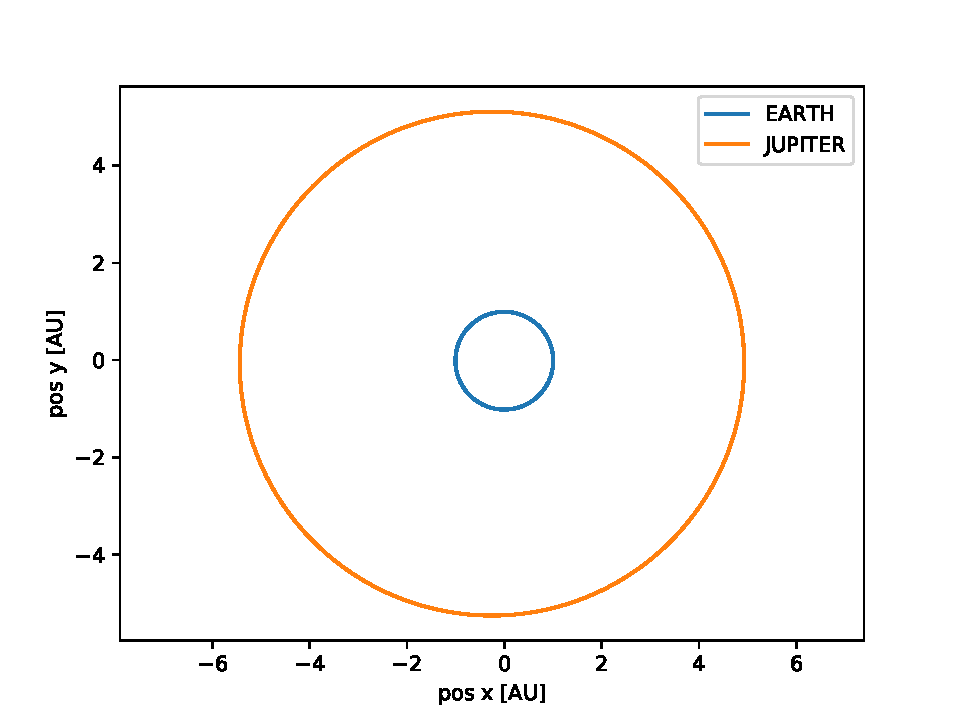
\includegraphics[scale=0.7]{../opp_e1.pdf}
		\caption{A plot of Jupiter and Earths path around the sun}
		%Label gjør det enkelt å referere til ulike bilder.
		\label{e_1}
\end{figure}

\begin{figure}[h!]
	\centering 
	%Scale angir størrelsen på bildet. Bildefilen må ligge i samme mappe som tex-filen. 
	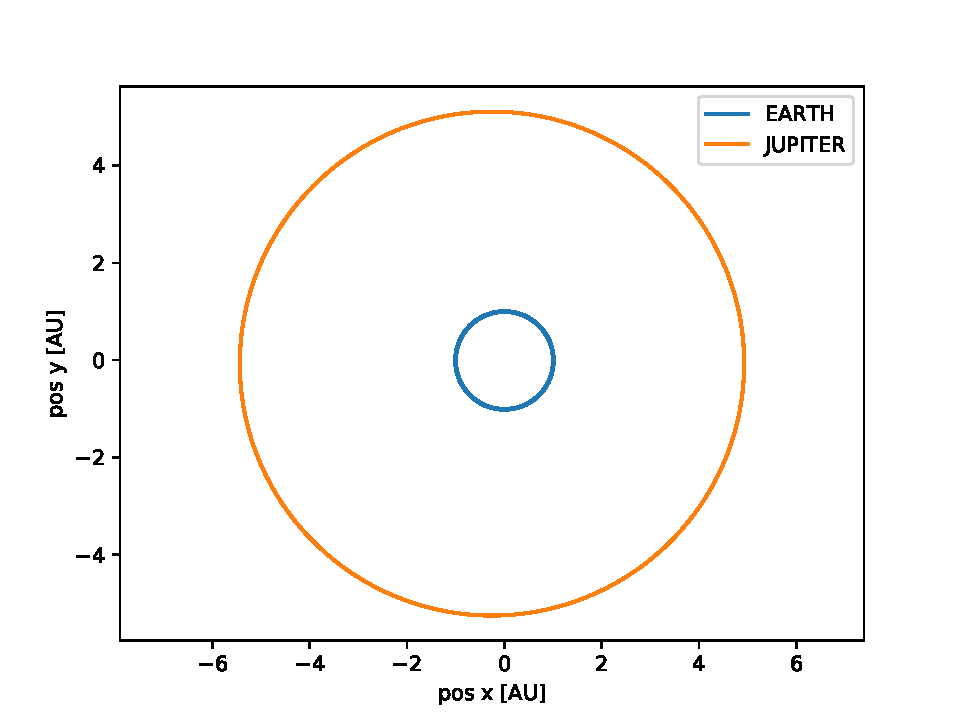
\includegraphics[scale=0.7]{../opp_e10.pdf}
	\caption{A plot of Jupiter and Earths path around the sun, when Jupiter has 10 times the mass}
	%Label gjør det enkelt å referere til ulike bilder.
	\label{e_10}
\end{figure}

\begin{figure}[h!]
	\centering 
	%Scale angir størrelsen på bildet. Bildefilen må ligge i samme mappe som tex-filen. 
	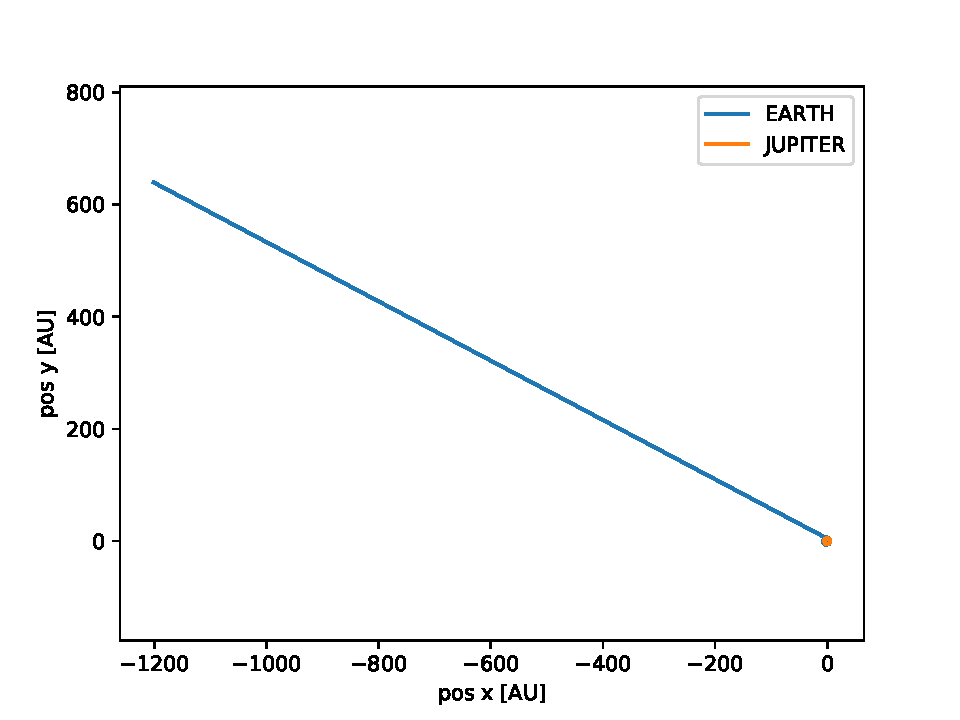
\includegraphics[scale=0.56]{../opp_e1000.pdf}
	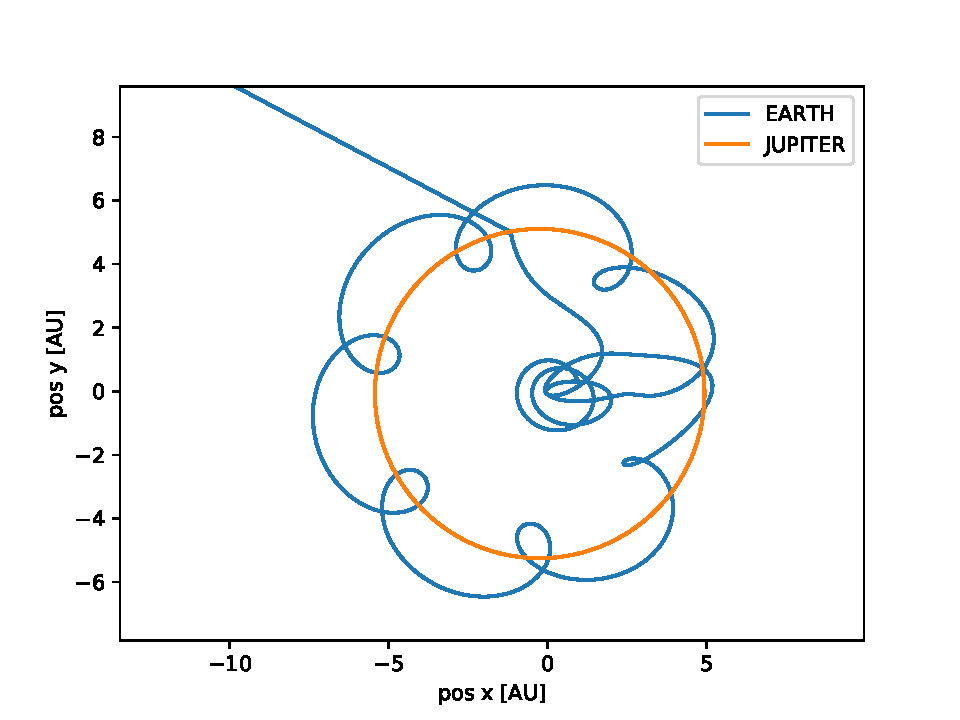
\includegraphics[scale=0.56]{../opp_e1000-0.pdf}
	\caption{A plot of Jupiter and Earths path around the sun, when Jupiter has 10000 times the mass}
	%Label gjør det enkelt å referere til ulike bilder.
	\label{e_1000}
\end{figure}

\subsection{Final model for all planets of the solar system}
The plot of the path of Jupiter, Earth and the Sun can be seen in figure \ref{f_0}, with an elapsed time of $t=20\text{yr}$ and a timestep of $10^{-5} \text{yr}$. The plot of the path of all the planets can be seen in \ref{f_1_0}, with an elapsed time of $t=300\text{yr}$ and a timestep of $10^{-3} \text{yr}$. The path of the planets closer to the centre can be seen in \ref{f_1_1}.

\begin{figure}[h!]
	\centering 
	%Scale angir størrelsen på bildet. Bildefilen må ligge i samme mappe som tex-filen. 
	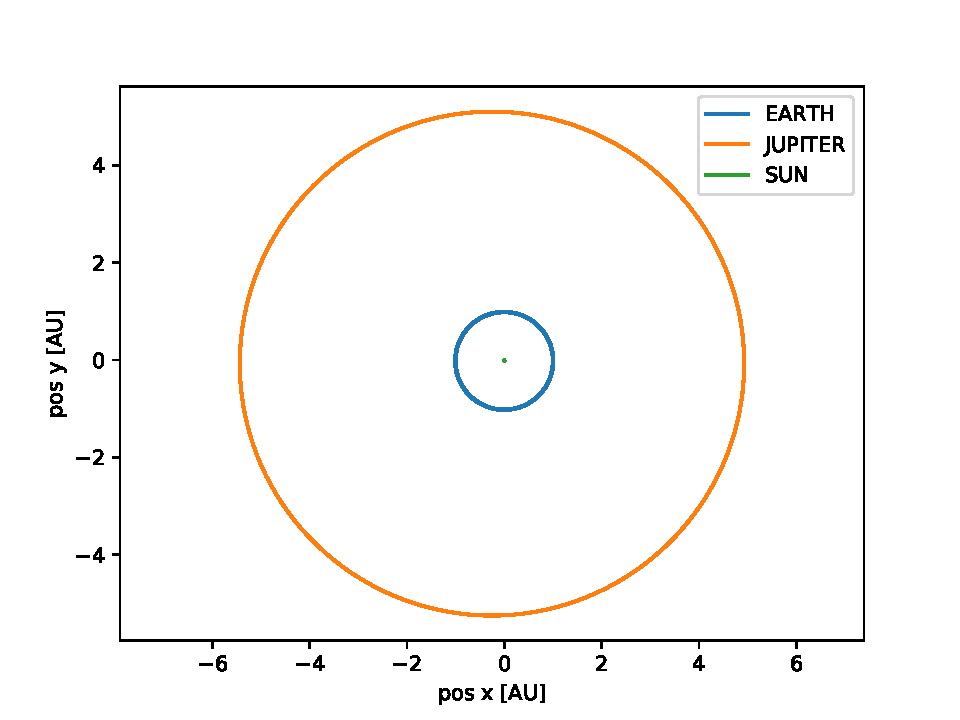
\includegraphics[scale=0.7]{../opp_f0.pdf}
	\caption{A plot of Jupiter, Earth and the Suns path around the centre of mass. You can't see it here, but the Sun moves in a small circle in the centre}
	%Label gjør det enkelt å referere til ulike bilder.
	\label{f_0}
\end{figure}

\begin{figure}[h!]
	\centering 
	%Scale angir størrelsen på bildet. Bildefilen må ligge i samme mappe som tex-filen. 
	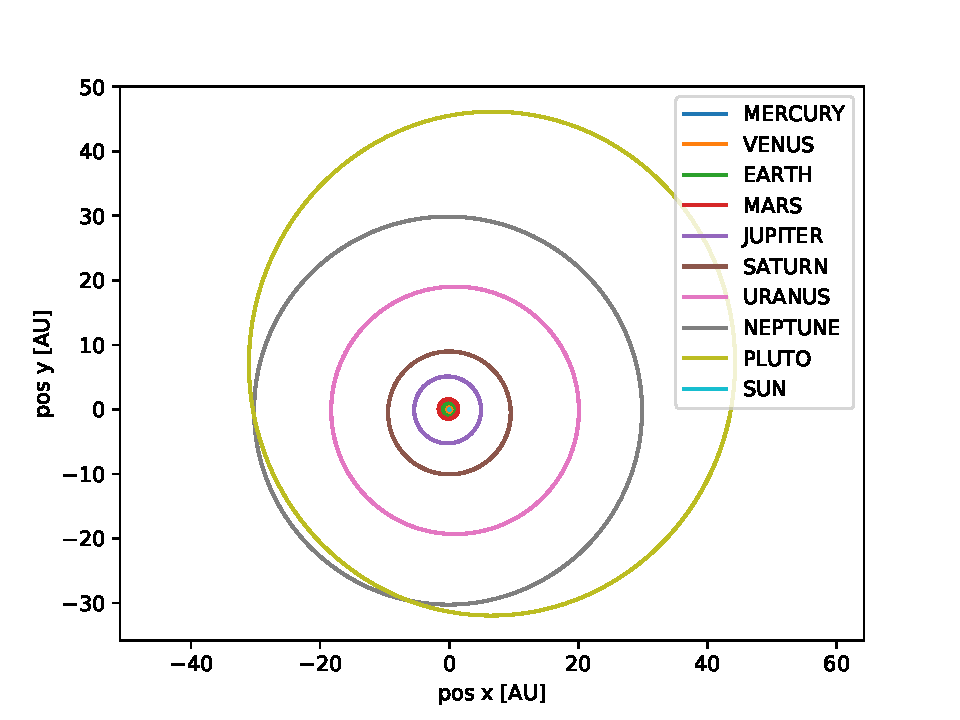
\includegraphics[scale=0.7]{../opp_f1.pdf}
	\caption{A plot of the Sun, all the planets and Plutos path around the centre of mass}
	%Label gjør det enkelt å referere til ulike bilder.
	\label{f_1_0}
\end{figure}

\begin{figure}[h!]
	\centering 
	%Scale angir størrelsen på bildet. Bildefilen må ligge i samme mappe som tex-filen. 
	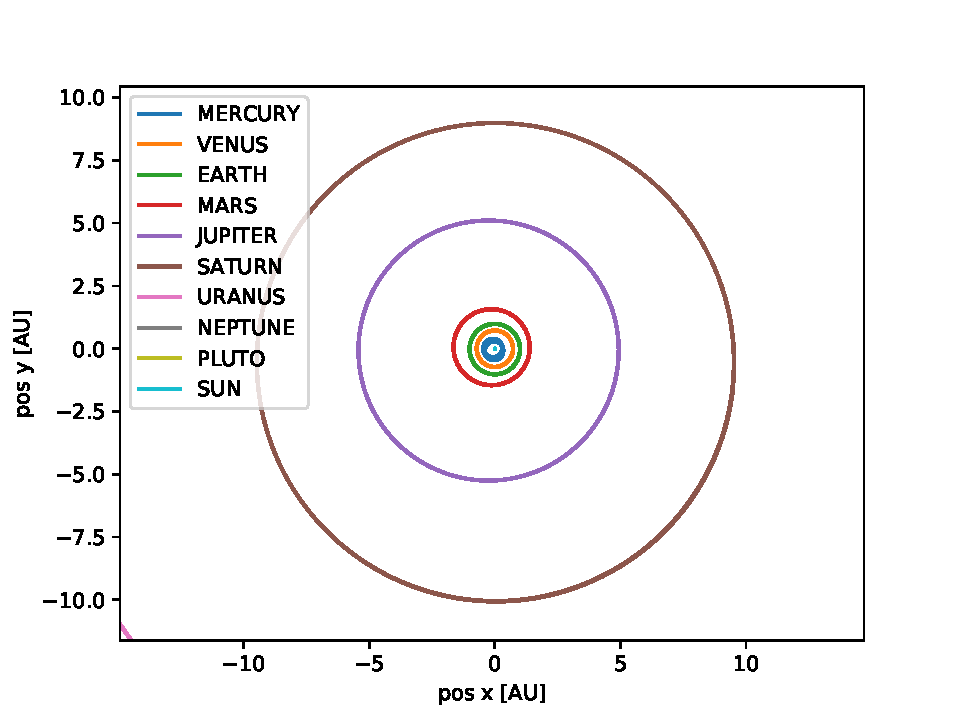
\includegraphics[scale=0.56]{../opp_f2.pdf}
	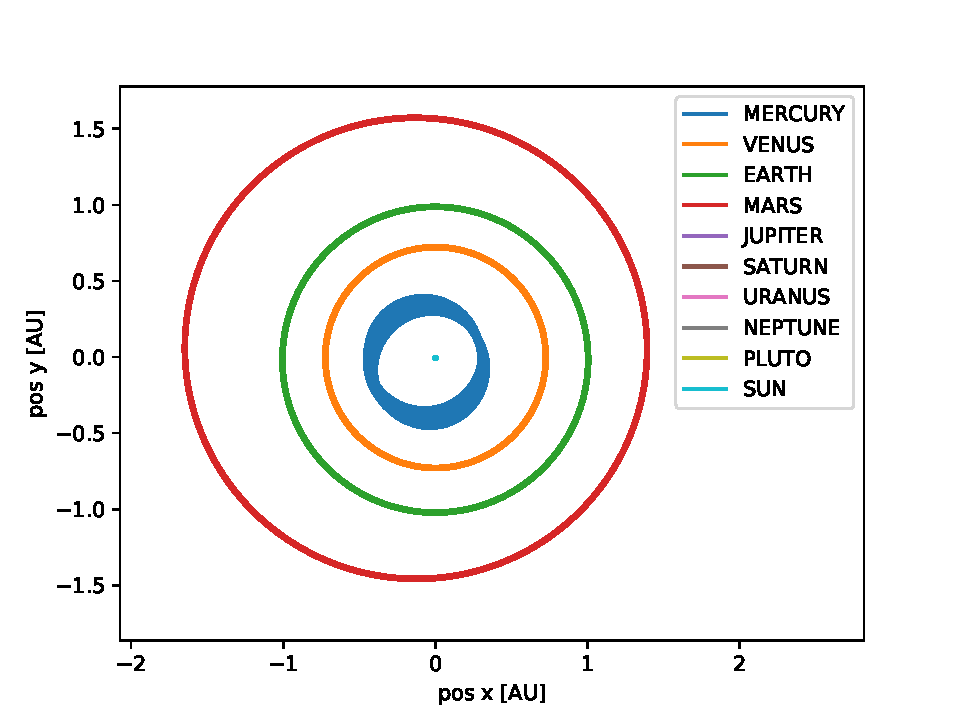
\includegraphics[scale=0.56]{../opp_f3.pdf}
	\caption{A plot of the Sun and the planets path around the centre of mass when we zoom in on the planets closer to the Sun}
	%Label gjør det enkelt å referere til ulike bilder.
	\label{f_1_1}
\end{figure}
\subsection{Testing the code}
As we can see quite clearly from figure \ref{escape_vel} that the planet leaves its orbit, and we can see from figure \ref{nescape_vel} that there is no room for reducing the initial velocity. This means that our code works as it should.

\subsection{Velocity Verlet vs Forward Euler}
When it comes to computation times the difference between the two methods is minimal, and a rough flop count confirms that they should be approximately equal. When it comes to accuracy there is a big difference however. Looking at the different runs in figure \ref{fe3d} and figure \ref{vv3d}, we can se that as time passes the orbit that should be stable widens quite a lot more for the Forward Euler simulation, than for the Velocity Verlet simulation.

\subsection{The three-body problem}
We see that the normal path of Earth and Jupiter are stable, suggesting that the Verlet algorithm we have created is a good aproximation. When Jupiters mass is 10 times stronger there is no noticeable difference in the path. When it is 1000 times stronger, Earth spins around the Sun and Jupiter a couple of times, before shooting out into space, while Jupiter has a stable orbit around the sun. This suggest that the Verlet method is good enough to simulate a stable path when Jupiters mass is 10 times stronger, but not when it is 1000 times stronger. This makes sense as when $1000M_{\text{Jupiter}}$ is about the same as $M_{\odot}$, which would make it pull on Earth as strongly as the Sun. If we hadn't fixed the Sun in the centre of mass, then it and Jupiter would either have an unstable orbit, or we would get something close to a Binary star system.

\subsection{Final model for all planets of the solar system}
In conclusion we see that our algorithm produces nice, stable orbits for all the planets. The only planet which seem to not be completley stable is the planet closest to the sun, Mercury, but this could just be that its path moves around more due to its closenes to the centre of mass. We can also se that we get a moon like effect between the Earth and Jupiter by increasing Jupiters mass significantly. This suggests that our algorithm should handle both moons and random asteroids as well as planets. All in all it seems like the Verlet method produced a good aproximation of our solar system.

\section{APENDICES}

\subsection{The Velocity Verlet method math}\label{vVerlet_math}

Firstly function \ref{velVerlet}:
\begin{align}
x_i^{(1)} = \frac{x_{i+1} - x_{i-1}}{2h} \Rightarrow 2hx_i^{(1)} &= x_{i+1} - x_{i-1} \\
x_{i-1} &= x_{i+1} - 2hx_i^{(1)}
\end{align}
\begin{align}
x_{i+1} &= 2x_i - x_{i-1} + h^2 x_i^{(2)} = 2x_i - \left( x_{i+1} - 2hx_i^{(1)} \right)  + h^2 x_i^{(2)} \\
2 x_{i+1} &= 2x_i + 2hx_i^{(1)} + h^2 x_i^{(2)} \\
x_{i+1} &= x_i + hx_i^{(1)} + \frac{h^2}{2} x_i^{(2)} 
\end{align}

Then function \ref{VvelVerlet}:
\begin{align}
x_{i+1} &= x_i + hx_i^{(1)} + \frac{h^2}{2} x_i^{(2)} \Rightarrow x_{i} = x_{i-1} + hx_{i-1}^{(1)} + \frac{h^2}{2} x_{i-1}^{(2)} \\
x_{i+1} &= x_{i-1} + hx_{i-1}^{(1)} + \frac{h^2}{2} x_{i-1}^{(2)} + hx_i^{(1)} + \frac{h^2}{2} x_i^{(2)} \\
x_i^{(1)} &= \frac{x_{i-1}^{(1)}}{2} + \frac{h}{4} x_{i-1}^{(2)} + \frac{x_i^{(1)}}{2} + \frac{h}{4} x_i^{(2)}
= x_{i-1}^{(1)} + \frac{h}{2} \left( x_i^{(2)} + x_{i-1}^{(2)} \right) 
\end{align}


\section{REFERENCES}
\begin{thebibliography}{9}
	\bibitem{lecture notes}
	Computational Physics, Lecture Notes Fall 2015, Morten Hjort-Jensen p.215-220
	\bibitem{nasa}
	\url{https://ssd.jpl.nasa.gov/?horizons#top}
\end{thebibliography}




%\begin{figure}[h!]
%	\centering 
%	%Scale angir størrelsen på bildet. Bildefilen må ligge i samme mappe som tex-filen. 
%	\includegraphics[scale=0.7]{opp2_7.pdf}
%	\caption{A plot of the entropy}
%	%Label gjør det enkelt å referere til ulike bilder.
%	\label{2.7}
%\end{figure}






















\end{document}